\documentclass[a4paper, 10pt, conference]{ieeeconf_de}


\overrideIEEEmargins

% See the \addtolength command later in the file to balance the column lengths
% on the last page of the document

\usepackage{float}
\usepackage{graphicx}
\usepackage{amsmath}
\usepackage{amssymb}
%\usepackage[latin1]{inputenc}
\usepackage[utf8]{inputenc}
\usepackage[ngerman]{babel}

\usepackage{fixltx2e}


\title{\LARGE \bf
	Histograms of Oriented Gradients for 3D Object Retrival
}

\author{Philipp Lambracht}


\begin{document}

\maketitle
\thispagestyle{empty}
\pagestyle{empty}


%%%%%%%%%%%%%%%%%%%%%%%%%%%%%%%%%%%%%%%%%%%%%%%%%%%%%%%%%%%%%%%%%%%%%%%%%%%%%%%%

\begin{abstract}

Die 3D Objekterkennung ist ein wichtiges Themengebiet der Mobilen Systeme und der autonomen mobilen Robotik geworden.
Ein populärer Ansatz um die Ähnlichkeit zwischen 3D Objekten zu bestimmen, sind globale Deskriptoren. Im Zuge
meiner Ausarbeitung für das Proseminar "`Mobile Systems Engineering"' habe ich den wissenschaftlichen Artikel 
"` Histograms of Oriented Gradients for 3d Object Retrieval"' von  Maximilian Scherer, Micheal Walter und Tobias Schreck 
ausgewählt und werde den darin beschriebenen und entwickelten  Deskriptor, im folgenden HOG3D genannt, genauer vorstellen.	

\end{abstract}

%%%%%%%%%%%%%%%%%%%%%%%%%%%%%%%%%%%%%%%%%%%%%%%%%%%%%%%%%%%%%%%%%%%%%%%%%%%%%%%%

\section{EINLEITUNG}

Zum Zeitpunkt der Veröffentlichung des von mir ausgewählten wissenschaftlichen Artikels wurden viele
unterschiedliche Methoden zur 3D Objekterkennung vorgestellt. Einzelne Deskriptoren konnten sich 
bisher nicht als überlegen herausstellen. Es hat sich etabliert, die jeweiligen Deskriptoren
geschickt zu kombinieren, um deren Stärken zu nutzen und somit eine weitaus bessere Ergebnisse bei der Objekterkennung zu erzielen.
Dementsprechend wird der in \cite{scherer2010histograms} vorgestellte 3DHOG mit hoch-dimensionalen Merkmal-Vektoren
verglichen und eine Kombination dieser beiden in einem Experiment versucht.
\newline
Hauptmotivation für der 3DHOG waren unter anderem bereits erfolgreiche Anpassungen von 2D-Bild-Analyse Methoden auf 3D Objekterkennung. Es wurde sich für die Anpassung des bereits erfolgreichen HOG aus \cite{dalal2005histograms} entschieden.


\subsection{Grundbegriffe}
Im folgenden werde ich ein paar wichtige Grundbegriffe für diese Ausarbeitung erläutern. 

\subsubsection{Globaler und partieller Ansatz}
Bei der 3D Objekterkennung gibt es zwei verschiedene Ansätze. Der globale Ansatz, zu dem der 3DHOG gehört, betrachtet jeweils die komplette Form des 3D Models und es wird nach Ähnlichkeiten gesucht, während der partielle Ansatz nach lokalen Ähnlichkeiten sucht. Als ähnlich werden 2 Objekte betrachten, wenn deren Merkmale einen Schwellenwert bezüglich ihrer Differenz bzw. Distanz unterschreiten. Ähnlichkeit ist in der 3D Objekterkennung problematisch, da zusätzlich zu gegebenenfalls sich unterscheidender Beleuchtung noch der Betrachtungswinkel eine Rolle spielt. Bisher konnte diese Problematik noch nicht absolut gelöst werden, weder für den globalen noch für den partiellen Ansatz. Dementsprechend haben entsprechende Lösungsversuche einen heuristische Natur \cite{scherer2010histograms}.

\subsubsection{Histogramm}
Histogramme dienen in der Statistik und Bildverarbeitung dazu, Häufigkeiten bestimmter Merkmale visuell darzustellen. Ein einfaches Beispiel aus der Bildverarbeitung wäre ein Histogramm eines
Graustufenbildes mit den jeweils darin vorkommenden Grauwerten. Ein Beispiel für eine grafische Darstellung ist bei \figurename~\ref{histo_pic} zu finden.

\begin{figure}[thpb]
	\centering
	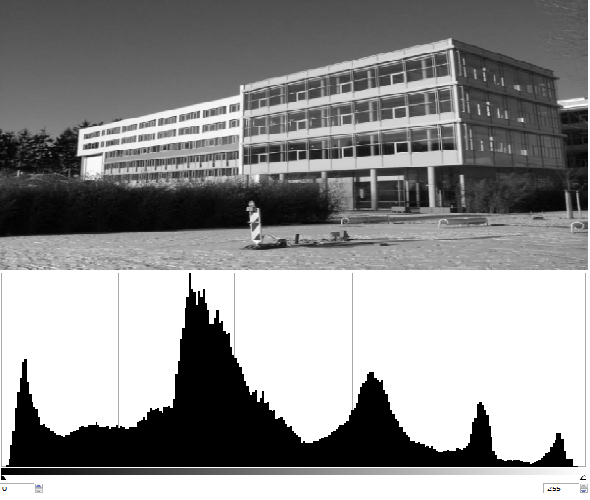
\includegraphics[width=\linewidth]{1-Einleitung/pics/pic_histo_uni01.png}
	\caption{Grauwertbild (entnommen aus Übungsmaterialien Bildverarbeitung 1 WS2015/2016) mit Histogramm (Erstellt mit GIMP 2.8.16)}
	\label{histo_pic}
\end{figure}


%\begin{table}[H]
%	\centering
%	\caption{Grauwert Histogramm}
%	\label{bsp Histogramm}
%	\begin{tabular}{ll}
%		Grauwert & Anzahl \\
%		150      & 30     \\
%		20       & 5      \\
%		...      & ...    \\
%		255      & 10    
%	\end{tabular}
%\end{table}

Eine detailreichere Einführung im Bezug auf Bildverarbeitung ist in \cite{Priese15} zu finden.

\subsubsection{Gerichtete Gradienten}
Gerichtete Gradienten werden wie z.B. in \cite{dalal2005histograms} äußerst erfolgreich zur Merkmaildetektion für 2D Bilder eingesetzt. Die Verwendung dieses Begriffs kann in \cite{scherer2010histograms} und dementsprechend in dieser Ausarbeitung vom mathematischen Begriff abweichen.
\newline
Um gerichtete Gradienten zu berechnen, benötigt man Gradientenoperatoren. Hiermit sind Lineare Filter aus der Bildverarbeitung gemeint. In der Einführungslektüre \cite{Priese15} versteht man Filter als Funktionen, welche auf Bilder, als Matrizen darstellbar, angewendet werden. Gradientenoperatoren sind gemäß der Definition über differenzierbare Funktionen, eine entsprechende Approximation mit denen man z.B. 2D Bilder "`ableiten"' kann. Die Filtermaske \ref{Abl_Maske} 

\begin{equation}
\label{Abl_Maske}
\begin{bmatrix}
-1 & 0 & 1
\end{bmatrix}
\end{equation}

bewirkt z.B. die 1. Ableitung. Dieser Filter kann z.B. für ein 2D Bild in die X-Richtung (Betrachtung der benachbarten Pixel links und rechts vom abzuleitenden Pixel) und in die Y-Richtung (Betrachtung der benachbarten Pixel über und unter dem Abzuleitenden Pixel) angewendet werden.  

\begin{table}[]
	\centering
	\caption{Grauwertbild als Matrix}
	\label{GrauwertMat}
	\begin{tabular}{llll}
		$a_{00}$ & $a_{01}$ & $a_{02}$ & $a_{03}$ \\
		$a_{10}$ & 100    & 50     & 235     \\
		$a_{20}$ & 73     & 42     & 150      \\
		$a_{30}$ & 30     & 125    & 0                     
	\end{tabular}
\end{table}

Formel \ref{abl_a22} zeigt ein Beispiel, wie ein Element aus \tablename~\ref{GrauwertMat} abgeleitet wird. In diesem Fall in X-Richtung. An den Rändern muss jeweils eine Randbehandlung vorgenommen werden. Werte können z.B. gespiegelt werden.
\begin{equation}
\label{abl_a22}
a_{22}'x = -73 + 0 +150 = 77
\end{equation}

Mit den Gradientenoperatoren lässt sich jeweils die Gradientenlänge bzw. -betrag und die Gradientenrichtung berechen. Die Formeln (\ref{Grad_L}) und (\ref{Grad_R}), entnommen aus \cite{Priese15} zeigen jeweils die Berechnung für 2D Bilder. $G_l$ ist der Gradientenbetrag und $G_r$ die Gradientenrichtung $I_x$ bzw. $I_y$ steht jeweils für die Ableitung in X- bzw. Y-Richtung. Mit dem Parameter p ist den entsprechende Pixel gemeint.
\begin{equation}
\label{Grad_L}
G_l(p) = \sqrt{I^2_x(p)+ I^2 y(p)}
\end{equation}

\begin{equation}
\label{Grad_R}
G_r(p) = arctan_2(- I_y(p),I_x(p))
\end{equation}


\subsubsection{3D Mesh}
3D Meshes werden dazu verwendet um 3D Objekte digital zu speichern. Es werden Informationen über die Vertices (Punkte), Kanten, Flächen, Polygone sowie falls nötig Informationen über die Oberfläche (z.B. Farbe) gespeichert. In dem ausgewählten Artikel \cite{scherer2010histograms} werden Meshes aus schon bestehenden Performanz-Tests genommen um die Leistungsfähigkeit des 3DHOG zu messen.	

\section{HAUPTTEIL}

In diesem Abschnitt werde ich zunächst den 2DHOG aus \cite{dalal2005histograms} kurz vorstellen, mit dem Hauptthema 3DHOG fortfahren und zuletzt das in \cite{scherer2010histograms} durchgeführte Experiment aufgreifen.

\subsection{2DHOG}
Im Bereich der 2D Objekterkennung aus Bildern existieren bereits erfolgreiche Methoden. Der Skale-Invariant-Feature-Transform Algorithmus (SIFT),genauere Beschreibung z.B. in \cite{Priese15}
zu finden, arbeitet mit aggregierten Gradienten. Beim 2DHOG werden hingegen die Gradienten entsprechend
ihrer Richtung in Histogrammen eingeordnet.
\newline
Die Idee hinter dem 2DHOG ist, dass sich Form und Aussehen von Objekten mit Gradienten beschreiben lassen.
Dies ist selbst möglich, ohne die genaue Position der Gradienten zu kennen. Der 2DHOG läuft grob nach folgenden Schema ab. Zuerst werden die Farbwerte des Bilds,auf dem die Detektion durchgeführt wird, normalisiert. Danach wird das Bild in gleich große, rechteckige Zellen aufgeteilt. Dabei können einzelne Zellen überlappen. Für jede dieser Zellen werden Histogramme für die jeweils berechneten Gradienten angelegt. Die Einteilung erfolgt entsprechend ihrer Richtung. Die Ergebnisse müssen normalisiert werden. Die HOGs werden mittels Detektionsfenster extrahiert und an eine Support Vector Machine (SVM) weitergeben. Danach kann entschieden werden, ob das entsprechende Objekt gefunden wurde. Im Fall von \cite{dalal2005histograms} Menschen. In dem eben genannten Wissenschaftlichen Artikel hat sich durch Experimente herausgestellt, dass die einfache Ableitungsmaske \ref{Abl_Maske} zur Berechnung der Gradienten die besten Ergebnisse liefert. 
Es wurden andere Ableitungsfilter, wie z.B. der Sobel-Operator (Formel \ref{Sobel}, entnommen aus \cite{Priese15}), jedoch waren die Ergebnisse eher enttäuschend. 

\begin{align}
\label{Sobel}
	S_x =	\begin{bmatrix}
				-1 & 0 & 1 \\
				-2 & 0 & 2 \\
				-1 & 0 & 1 
			\end{bmatrix}  &  
	S_y =	\begin{bmatrix}
				-1 & -2 & -1 \\
				 0 & 0 &   0 \\
				 1 & 2 &   1 
			\end{bmatrix}	
\end{align}
Auch wurde, zwecks Optimierung, mit Gaußfiltern experimentiert. Eine Performenceverbesserung wurde ebenfalls nicht erzielt. 
Detailliertere Informationen über den 2DHOG sind in \cite{dalal2005histograms} zu finden.

\subsection{3DHOG}


\subsubsection{Erweiterung des 2DHOG auf 3DHOG}
Der erste Schritt, die Berechnung der Gradienten, erweist sich bei der Erweiterung auf 3DHOG ein wenig komplizierter. Zunächst Benötigt man eine Notation für Nachbarschaft und Intensität für die Polygon Meshs. In \cite{scherer2010histograms} wird dafür ein dreidimensionales euklidisches 
Distanzfeld berechnet. Dieses Feld ist als eine reellwertige Funktion aufzufassen, welche auf einem diskreten, regulären 3D Gitter definiert ist. Das Gitter umfasst dabei das komplette Volumen des Meshs \cite{scherer2010histograms}. Die jeweiligen Gitterzellen können auch als Voxel bezeichnet werden. Jeder Voxel enthält dabei die Information über den Abstand seines Zentrums zur Oberfläche des Meshs. 

\begin{equation*}
f: \mathbb{N} \times \mathbb{N} \times \mathbb{N} \mapsto \mathbb{R} 
\end{equation*}
\begin{equation}
\label{Distanzfeld_Fkt}
f(x,y,z) = \min_{\substack{x \in \Sigma}} \| x-center(x,y,z) \|_2
\end{equation}
Eine Definition der Funktion ist bei Formel (\ref{Distanzfeld_Fkt}) zu sehen, entnommen aus \cite{scherer2010histograms}. $\Sigma$ ist hierbei die Menge aller Punkte auf der Oberfläche des Meshs und $center: \mathbb{N} \times \mathbb{N} \times \mathbb{N} \mapsto p $ liefert die Koordinate des Zentrums des Voxels zurück.
\newline
Auf das berechnete Distanzfeld kann man z.B. die Filtermaske $\begin{bmatrix} -1 & 0 & 1\end{bmatrix}$ aus \cite{dalal2005histograms} anwenden für die Gradientenberechnung.
\newline
Das Distanzfeld wird sehr stark von Position und Größe des Objekts beeinflusst. Dementsprechend muss das Mesh vor der Distanzfeldberechnung normalisiert werden. In \cite{scherer2010histograms} greift man deshalb auf Translationsinvarianz  (das Zentrum der Masse des Meshs wird in den Ursprung verlegt), Skalierungsinvarianz (Skallierung des Meshs in den Einheitswürfel), sowie eine Normalisierung für Rotation mittels gewichteter PCA analyse.
\newline
Der zweite Schritt ist um weiten simpler. Die dreidimensionalen Gradienten werden jeweils entsprechend ihrer Richtung in Histogramme für die einzelnen Zellen eingeordnet. Hierfür werden die Gradienten in sphärische Koordinaten entsprechend Formel (\ref{Sphere_Koord}), entnommen aus \cite{scherer2010histograms}, umgerechnet.

\begin{equation}
\label{Sphere_Koord}
\begin{pmatrix}
	\theta \\ 
	 \phi \\ 
	 r
\end{pmatrix}
= \begin{pmatrix}
	\arccos\dfrac{z}{\sqrt{x^2+y^2+z^2}} \\ 
	 atan2(x,y) \\ 
	 \sqrt{x^2+y^2+z^2}
\end{pmatrix}
\end{equation}
Die Einordnung erfolgt entsprechend ihrer Richtung ($Zenit \theta \in [0,\pi) $ und $Azimut \phi \in [0,2\pi)$)  

\subsubsection{3DHOG Extraktionsalgorithmus }
Der schematische Ablauf des Extraktionsalgorithmus ist in \figurename~\ref{Vekt_ext_pipe} zu sehen. Genaueres über die Implementation ist in dem in \cite{scherer2010histograms} mitgelieferten Sourcecode \footnote{www.gris.informatik.tu-darmstadt.de/projects/vsa/3dhog/3dhog.zip} zu entnehmen 

 \begin{figure}[thpb]
 	\centering
 	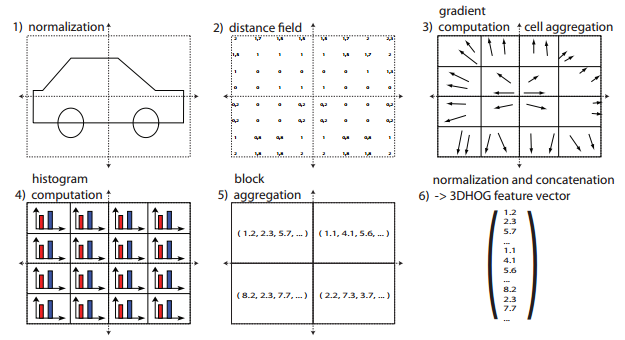
\includegraphics[width=\linewidth]{2-Hauptteil/pics/3DHOG_extrac_pipe.png}
 	\caption{Vektor Extraktionspipeline aus \cite{scherer2010histograms}}
 	\label{Vekt_ext_pipe}
 \end{figure}
 
\subsection{Experiment}
Im folgenden werde ich das in \cite{scherer2010histograms} durchgeführte Experiment und dessen Ergebnisse vorstellen. Um die Effizienz der Deskriptoren zu vergleichen werden Precision-and-recall-Diagramme verwendet

\subsubsection{Verwendete Benchmarks}
Für das Experiment wurden drei etablierte Benchmarks genommen, welche 3D Mesh Modelle enthalten. Der Princton Shape Benchmark (PSB), 2009 SHREC Generic Shape Retrieval Contest dataset (SHREC) und Konstanz 3D shape database (KN-DB). Die einzelnen 3D Modelle sind in verschiedene Klassen eingeteilt (z.B. Menschen, Tiere, Autos, .. ), damit verschiedene 3D Deskriptoren besser miteinander verglichen werden können. Je nachdem um welche Objektart es sich handelt, liefern Deskriptoren unterschiedlich gute Ergebnisse. 

\begin{table}[H]
	\centering
	\caption{}
	\label{Benchmarks}
	\begin{tabular}{lllll}
		Benchmark & anz. Modelle & anz. Klassen & durchschn. anz. M. pro K. &  \\
		PSB       & 1814         & 92           & 10                                 &  \\
		KN-DB     & 473          & 55           & 9                                  &  \\
		SHREC     & 720          & 40          & 18                                & 
	\end{tabular}
\end{table}
\subsubsection{Verwendete Vergleichsdeskriptoren}
Im folgenden werde ich die Vergleichsdeskriptoren kurz anreißen. Details sind in \cite{dvvra3DModelret} zu finden.

\paragraph{438-dimensional Depth-Buffer Descriptor (DBD438)}
Dieser Deskripter nutzt das aus der Computergrafik bekannte Tiefenpufferverfahren. Nach \cite{scherer2010histograms} gilt dieser Deskriptor als einer der effektivsten.

\paragraph{300-dimensional Silhoutte-based Descriptor(SIL300)}
Der SIL300 arbeitet mit der Zerlegung des 3D Models in 2D Silhouetten 
mit den jeweiligen Achsen (y,z) (z,y) und (x,y).

\paragraph{136-dimensional Descriptor based on Radial Extent function (RSH136) }
Bei diesem Deskriptor wird mit der Ausdehnung von 3D Objekten gearbeitet. Die Objekte werden entlang gegebenen Richtungen(entlang von vorher definierten Strahlen) gemessen.

\paragraph{472-dimensonal Hybrid Descriptor (DSR472) }
Hierbei handelt es sich um einen Hybrid aus den vorigen Deskriptoren. Da hier geschickt die einzelnen Stärken kombiniert werden, ist sogar dem DBD438 überlegen.

\subsubsection{Ergebnisse des Experiment}
Zunächst wurde überprüft, ob sich zur Gradientenberechnung ggf. Gradienten der 2. Ableitung (Formel \ref{Abl_''_Maske}) bessere Ergebnisse liefern.    
\begin{equation}
\label{Abl_''_Maske}
\begin{bmatrix}
1 & 0 & -2 & 0 & 1
\end{bmatrix}
\end{equation}
Da dies der Fall war, wurden alle weiteren Benchmarks mit der 2. Ableitung durchgeführt. Im Vergleich mit den einzelnen Deskriptoren schlägt sich der 3DHOG Relativ gut, schneidet sogar beim SHREC Benchmark besser als die anderen Deskriptoren ab (\figurename~\ref{Shrec_diag}).

 \begin{figure}[thpb]
 	\centering
 	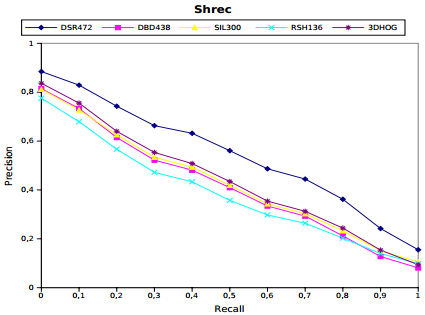
\includegraphics[width=\linewidth]{2-Hauptteil/pics/SHREC_diag.png}
 	\caption{SHREC Precision-Recall-Diagramm aus \cite{scherer2010histograms}}
 	\label{Shrec_diag}
 \end{figure}
 
 Entsprechend wenig überraschend ist er aber dem Hybrid Deskriptor unterlegen. Dennoch schneidet der 3DHOG beim SHREC Benchmark bei einzelnen Klassen besser ab, als der Hybrid. Zu sehen in \figurename~\ref{SHREC_3DHOG_DSR472} 

 \begin{figure}[thpb]
 	\centering
 	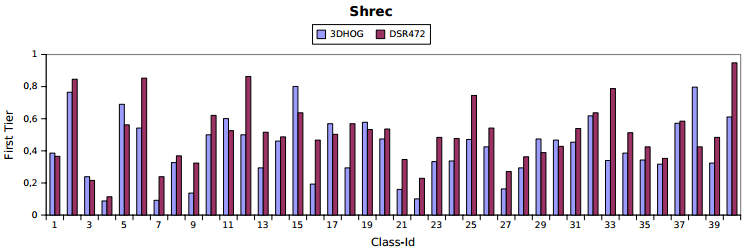
\includegraphics[width=\linewidth]{2-Hauptteil/pics/SHREC_3DHOG_DSR472.png}
 	\caption{1. Tier Präzision der verschieden Klassen des SHREC Benchmark aus \cite{scherer2010histograms}}
 	\label{SHREC_3DHOG_DSR472}
 \end{figure}
 
 Dies legt nahe, dass der 3DHOG wichtige 3D Merkmale erkennt, die den anderen Deskriptoren entgehen \cite{scherer2010histograms}.
\newline
Entsprechende Versuche, in denen der 3DHOG mit dem DSR472 kombiniert wurde führten zu einer Performanceverbesserung, wie in \figurename~\ref{SHREC_TEAM_3DHOG_DSR472} zu sehen. 

\begin{figure}[thpb]
	\centering
	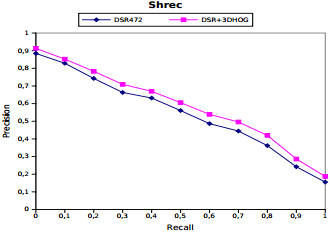
\includegraphics[width=\linewidth]{2-Hauptteil/pics/SHREC_TEAM_3DHOG_DSR472.png}
	\caption{SHREC Precision-Recall-Diagramm aus \cite{scherer2010histograms}}
	\label{SHREC_TEAM_3DHOG_DSR472}
\end{figure}

Der 3DHOG stellt damit einen wertvollen Beitrag zur Verbesserung von 3D Objekterkennungssystemen da \cite{scherer2010histograms}.



\section{DISKUSSION}
Dieser Abschnitt befasst sich mit den optimalen Parametern des 3DHOG, welche sich aus dem Experiment aus \cite{scherer2010histograms} ergeben hat. Außerdem wird auf ein dort eingetreten Problem bei der Gradientendefinition eingegangen.
\subsection{Parameterwahl des 3DHOG}
Das Experiment von Scherer, Walter und Schreck in \cite{scherer2010histograms} hat gezeigt, dass die Parameterwahl für den 3DHOG die Performanz stark beeinflussen kann. Eine als optimal erwiesene Einstellung ist in \figurename~\ref{Parameter} zu finden.

\begin{table}[H]
	\centering
	\caption{Optimale Parameterwahl für 3DHOG, entnommen aus \cite{scherer2010histograms}}
	\label{Parameter}
	\begin{tabular}{ll}
		Parameter                & Wert     \\
		r\textsubscript{x,y,z} & $\frac{2}{52}$    \\
		c\textsubscript{x,y,z} & 12 vxl   \\
		bins($ \theta $)       & 9        \\
		bins($ \phi $)         & 9        \\
		b\textsubscript{x,y,z} & 2 Zellen \\S
		o\textsubscript{x,y,z} & 0 Zellen \\
		Dimensionalität          & 5184    
	\end{tabular}
	
\end{table}

Der Parameter r\textsubscript{x,y,z} legt die Anzahl der Voxel im Distanzfeld fest. r\textsubscript{x,y,z} steht jeweils für die Kantenlänge jedes Voxels. Je kleiner die Kantenlänge gewählt wird, desto weniger Informationen gehen verloren, jedoch erhöht sich die Rechenzeit. Mit der Zellengröße c\textsubscript{x,y,z} stellt man ein, wie viele Gradienten in ein Histogramm aufgenommen werden. Damit lässt sich der Grad der Lokalität des Deskriptors konfigurieren \cite{scherer2010histograms}.
Mit den Parametern 	bins($ \theta $) und bins($ \phi $) bestimmt die Feinheit der Einteilungen des Histogramms. Hier hat man die Wahl zwischen Genauigkeit und Stabilität.
Die nächsten beiden Parameter legen jeweils die Größe der Blöcke (b\textsubscript{x,y,z})  und ihre Überlappung  (o\textsubscript{x,y,z}) fest. Damit wird konfiguriert, wie viele benachbarte Zellen miteinander normalisiert werden. Diese beiden Parameter wurden entsprechend vielversprechenden Parameter aus \cite{dalal2005histograms} gewählt. Die Überlappung hatte jedoch nicht den erwarteten positiven Effekt. Deshalb wurde der Wert 0 gewählt.


\subsection{Alternative Gradientendefinition}
Durch Experimentieren hat sich herausgestellt, dass sich die zweite Ableitung für die Gradientenberechnung des 3DHOG als effektiver erwiesen hat. Scherer, Walter und Schreck \cite{scherer2010histograms} begründen es damit, dass nicht nur Informationen über Lokale Extrema in der Nähe Oberfläche des Meshes, sondern auch Informationen innerhalb des Meshs nützlich sein können. 
 \begin{figure}[thpb]
 	\centering
 	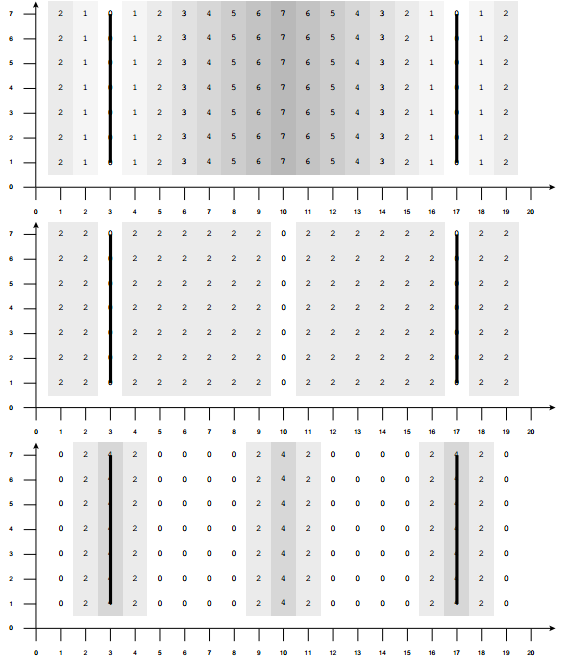
\includegraphics[width=\linewidth]{3-Diskussion/pics/2D_distance_field.png}
 	\caption{2D Darstellung eines Distanzfeldes, entnommen aus \cite{scherer2010histograms}. Das oberste Bild zeigt das eigentliche Distanzfeld, das Mittlere unter Verwendung der ersten Ableitung, das untere mit der zweiten Ableitung}
 	\label{2D_distance_field}
 \end{figure}
 Zudem liefert die ersten Ableitung nicht genau das, was man unter Gradienten in der Bildverarbeitung versteht. Einen Pixel kann man als einen Punkt in der Welt verstehen, in dem Informationen über das reflektierte Licht gespeichert werden. Der entsprechende Gradient würde z.B. an Ecken von Wänden an Stärke zunehmen. \figurename~\ref{2D_distance_field} zeigt deutlich, dass dies bei der ersten Ableitung nicht der Fall ist. Die 2. Ableitung hingegen erfüllt die Grundauffassung von Gradienten in der Bildverarbeitung.
 \newline
 
 
   

\addtolength{\textheight}{-12cm}  % This command serves to balance the column lengths
                                  % on the last page of the document manually. It shortens
                                  % the textheight of the last page by a suitable amount.
                                  % This command does not take effect until the next page
                                  % so it should come on the page before the last. Make
                                  % sure that you do not shorten the textheight too much.

%%%%%%%%%%%%%%%%%%%%%%%%%%%%%%%%%%%%%%%%%%%%%%%%%%%%%%%%%%%%%%%%%%%%%%%%%%%%%%%%

% References (BibTeX)
\bibliographystyle{plain}
\bibliography{paper}

\end{document}
